\style{plain}

\section{À propos de la carte \mb}


\mb est un microcontrôleur développé au Royaume-Unis.
Par ses caractéristiques techniques et ses interfaces
pédagogiques, cet objet possède un fort potentiel pour
l’enseignement de l’algorithmique.



\begin{wrapfigure}{r}{4cm}
	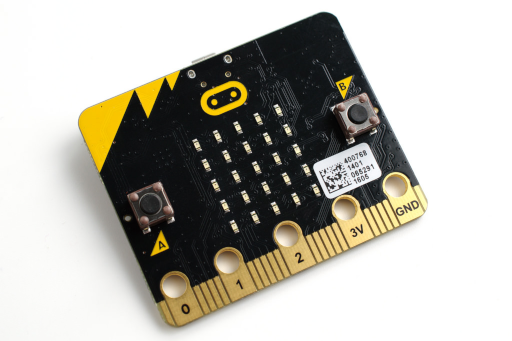
\includegraphics[width=\linewidth]{res/mb-ap-01.png}
	\legend{Carte \mb}
\end{wrapfigure}

Après un bref rappel historique, nous expliquerons plus en détail les caractéristiques propres de cet objet. Nous mettrons ensuite en avant la facilité de mise en œuvre en formation puis nous poursuivrons en donnant un premier aperçu de l’intérêt pédagogique de \mb.

\subsection{Bref historique}


Le développement de \mb s’inscrit dans le cadr d’une politique volontariste de développement de l’apprentissage de la programmation. L’objectif premier visait à équiper tous les élèves de 11/12 ans du Royaume-Unis ainsi que leur enseignant. Maintenant que c’est chose faite, le reste du monde peut en profiter aussi.

% \begin{wrapfigure}[12]{r}{5cm}
%     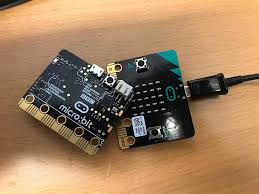
\includegraphics[width=\linewidth]{res/mb-ap-03}
%     \legend{Cartes \mb branchée en USB}
% \end{wrapfigure}


La BBC\footnote{Make It Digital - The BBC micro:bit. (s. d.). Consulté 29 mars 2017, à l’adresse \url{http://www.bbc.co.uk/programmes/articles/4hVG2Br1W1LKCmw8nSm9WnQ/the-bbc-micro-bit}} est le moteur de ce projet. 30 ans après sa première distribution d’ordinateurs aux enfants britanniques\footnote{BBC Micro. (2016, septembre 20). In Wikipédia. Consulté à l’adresse \url{https://fr.wikipedia.org/w/index.php?title=BBC_Micro&oldid=129763631}}, “la Vieille Dame” remet ça aujourd’hui. La BBC utilise ses moyens de diffusions pour promouvoir et accompagner les utilisateurs, notamment en proposant des émissions de TV dédié à cet objet sur un mode ludique et divertissant. Sur les 29\footnote{Partners. (s. d.). Consulté 29 mars 2017, à l’adresse \url{https://www.microbit.co.uk/partners}} partenaires de ce projet, se trouvent entre autres Microsoft\footnote{The BBC micro:bit and Microsoft - Microsoft Research. (s. d.). Consulté 29 mars 2017, à l’adresse \url{https://www.microsoft.com/en-us/research/project/the-bbc-microbit-and-microsoft/}} pour une partie logiciel et interface de programmation, ARM\footnote{Ltd, A. R. M. (s. d.). ARM | Innovation Hub - BBC micro:bit. Consulté 29 mars 2017, à l’adresse \url{http://www.arm.com/innovation/products/microbit.php}} pour la construction des processeur et la partie matériel, et Samsung\footnote{Code on the go with Samsung \& micro:bit. (s. d.). Consulté 29 mars 2017, à l’adresse \url{http://www.samsung.com/uk/citizenship/bbcmicrobit.html}} pour un support mobile. C’est donc un projet qui mobilise des acteurs majeurs du numériques et de la communication, prévu pour durer.

% \begin{figure}
%     \center
%     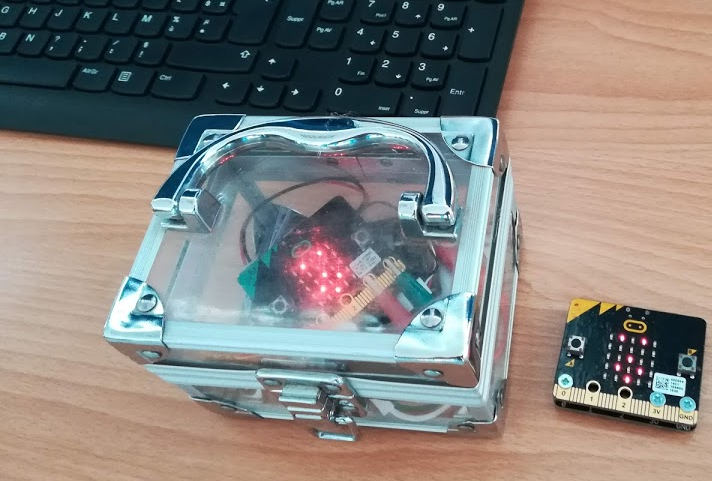
\includegraphics[width=0.5\linewidth]{res/mb-ap-02}
%     \legend{Cartes \mb lors d'un escape game utilisé en formation}
% \end{figure}


\subsection{La carte \mb}

Concrètement de quoi s’agit-il ? On parle ici de microcontrôleur, à savoir une carte électronique programmable pour interagir avec le monde réel.
C’est une version accessible de l’électronique que tout un chacun manipule au quotidien sans se poser de question, par exemple les dispositifs de domotique qui permettent de gérer à distance le chauffage, la sécurité, l’arrosage du géranium… Ou bien plus simplement la bouilloire programmable au degré ${}^{\circ}$C près, la guirlande du sapin qui clignote au rythme de Jingle Bells. 
Ce microcontrôleur permet d’élaborer par exemple un podomètre, un doudou sensoriel, un sismographe rudimentaire\ldots

\begin{figure}
    \centering
    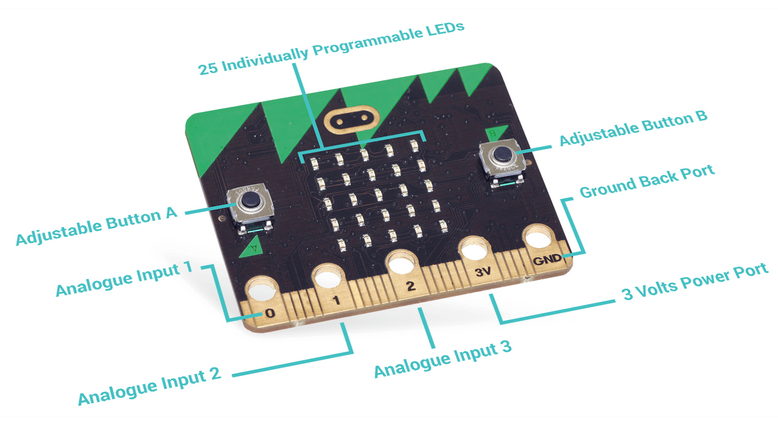
\includegraphics[width=0.49\linewidth]{res/mb-ap-04}
    \hfill
    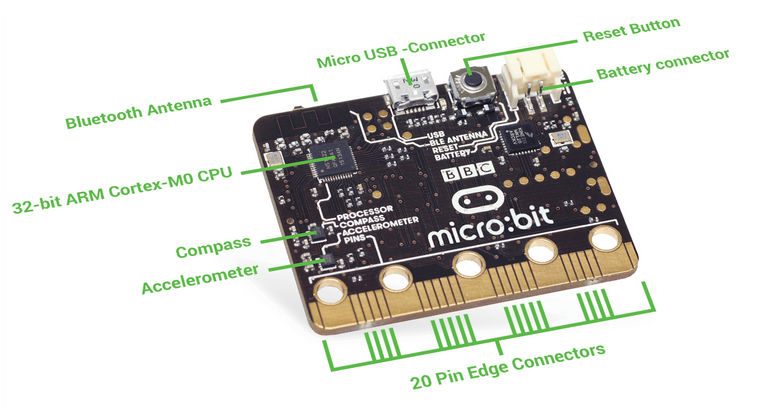
\includegraphics[width=0.49\linewidth]{res/mb-ap-05}
    \legend{Détails des entrées/sorties d'une carte \mb}
\end{figure}

L’interface de programmation est conçue pour être utilisable par un enfant d’une dizaine d’année, c’est donc la simplicité qui prime. On dispose en première approche d’une application internet utilisant le principe de la programmation par bloc, à savoir sur le principe des Blockly que l’on retrouve dans Scratch ou StudioCode. En plus d’une programmation accessible, l’interface propose une simulation de la carte. Ceci permet de voir directement les effets du programme dans l’interface. Pour un usage plus avancé il est notamment possible de programmer avec le langage Python\footnote{Python editor. (s. d.). Consulté 29 mars 2017, à l’adresse \url{http://python.microbit.org/editor.html}} ou Javascript.


\begin{minipage}[b]{0.45\linewidth}
    \vspace{0cm}
    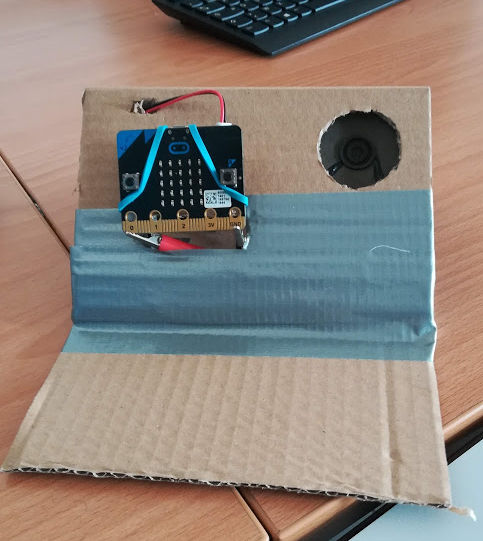
\includegraphics[width=\linewidth]{res/mb-ap-07}
    \legend{Cartes \mb qui fait de la musique (stage 2018)}
\end{minipage}
\hfill
\begin{minipage}[b]{0.45\linewidth}
    Bien entendu de nombreux exemples de projets existent, qu’ils soient issus des émissions BBC ou de la communauté éducative. Sur le site officiel on trouve des idées, des tutoriels, des leçons\footnote{Idées | micro:bit. (s. d.). Consulté 29 mars 2017, à l’adresse \url{http://microbit.org/fr/ideas/}} comme par exemple : une alarme de trousse, un compteur de frappe (au baseball) ou encore des leçons sur l’accélération.
    \vspace{1em}
    \begin{center}
        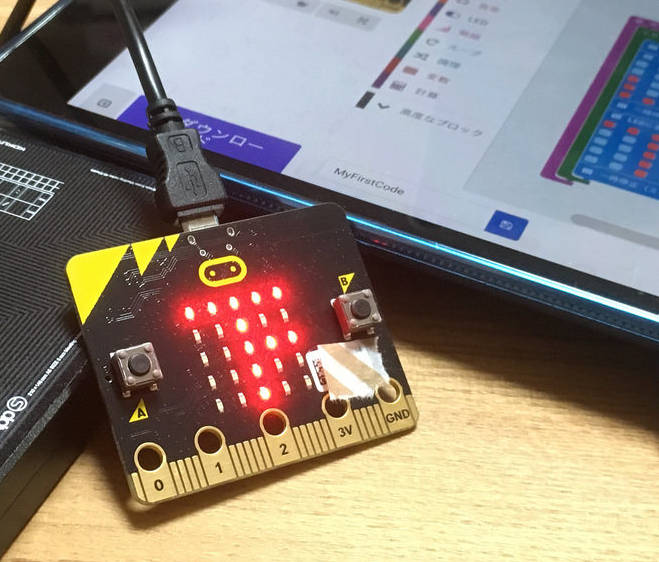
\includegraphics[width=\linewidth]{res/mb-ap-08}
    \end{center}
\end{minipage}


\subsection{Programmer la carte \mb \emph{par blocs}}

\subsubsection{Une interface en ligne}

L’interface de programmation par blocs a été développée en partenariat avec microsoft, elle se trouve en ligne à cette adresse: \url{https://makecode.microbit.org}

Il s’agit donc d’une page internet mais dont le code est mis en cache par le navigateur ce qui signifie qu’elle reste opérationnelle hors ligne.


\begin{remarque}
    À partir de chrome par exemple, il est possible de créer un raccourci sur le bureau.
\end{remarque}



\subsubsection{Un simulateur !}

Le très gros intérêt de cette interface consiste en son simulateur de carte qui permet d’avoir un aperçu du fonctionnement du programme avant même de le télécharger sur la carte.

\begin{figure}[h]
    \centering
    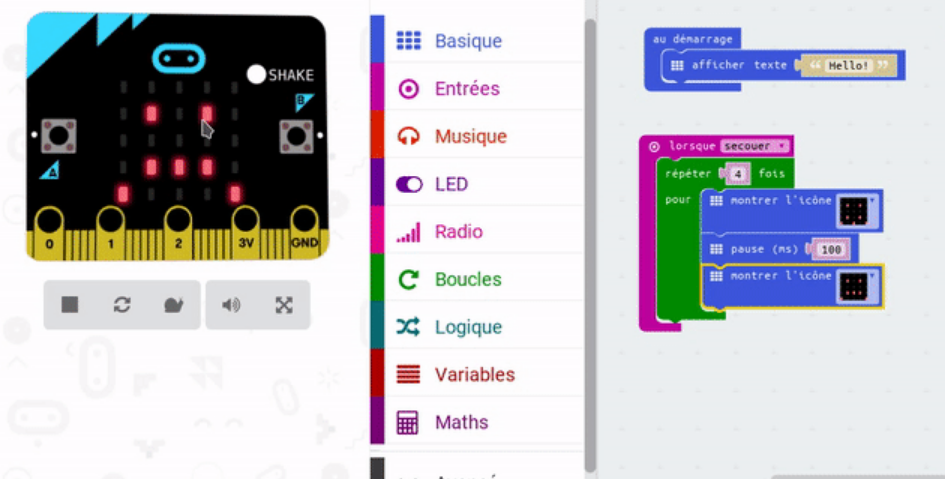
\includegraphics[width=0.75\linewidth]{mb-prog.png}
    \legend{Interface de programmation par bloc qui intègre un \emph{simulateur}}
\end{figure}




\begin{remarque}
    Le simulateur peut ne pas fonctionner hors ligne.
\end{remarque}

\subsubsection{Compilation et enregistrement}

Le téléchargement sur la carte se fait très simplement puiqu’elle est reconnue comme une clé USB. Il suffit donc de cliquer sur Télécharger et de copier le fichier obtenu (.hex) sur la carte.

\subsubsection{Programmation par bloc}

Comme toute interface de programmation par blocs, elle est très intuitive à manipuler. Les premiers programmes se font très simplement et les catégories sont classées par couleurs et par technicité.

\begin{remarque}
    L’interface propose aussi de programmer en javascript, il suffit juste de cliquer sur un bouton pour changer de type de programmation.
\end{remarque}

\subsubsection{Documentation}

\begin{itemize}
    \item Une page de documentation présente les éléments de base pour la programmation par blocs\\
        \url{https://makecode.microbit.org/blocks}
    \item Une page de références présentent quelques fonctionnalités propre au microbit\\
        \url{https://makecode.microbit.org/reference}
\end{itemize}


\subsection{Programmer la carte \mb en \emph{Python}}

Le \mb peut exécuter une version allégée de Python qui s’appelle MicroPython. C’est une version spécialement dédiée aux microcontroleurs.

\subsubsection{Une interface en ligne}

Il est possible de programmer en python à partir d’un éditeur en ligne \url{http://python.microbit.org}

L’interface est cependant assez pauvre en fonctionnalité et ne dispose pas de l’autocomplétion.

\begin{figure}[h]
    \centering
    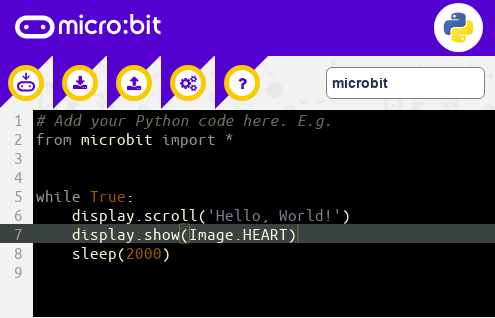
\includegraphics[width=0.65\linewidth]{res/mb-prog2.png}
    \legend{Interface de programmation en ligne}
\end{figure}

\subsubsection{Mu : une interface complète}

Comme le dit (en anglais) la page d’accueil de Mu : Mu est un éditeur de code simple pour les programmeurs débutants. Il est développé en Python et fonctionne sur Windows, OSX, Linux et Raspberry Pi.


\begin{figure}[h]
    \centering
    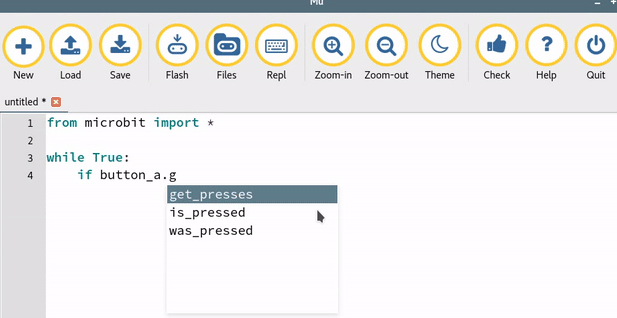
\includegraphics[width=0.65\linewidth]{res/mb-prog3.png}
    \legend{Interface de programmation Mu}
\end{figure}

\subsubsection{Programmation}

L’autocomplétion et l’autoindentation est très efficace. L’interface est rapidement utilisable par un débutant en programmation.
Compilation et enregistrement

Le téléchargement sur la carte se fait très simplement puisqu’il suffit de cliquer sur le bouton Flash . Il est tout de même préférable d’avoir au préalable le réflexe de vérifier le code avec Check .

\subsubsection{Communication série}

La fonction REPL de Mu permet d’ouvrir une communication via un port série avec le \mb. Il est ainsi possible d’envoyer et de recevoir des données. Sur les versions bêta il y a même un plotteur qui permet de visualiser graphiquement les données reçues.

\subsubsection{Documentation}

Il est existe un documentation sur microbit et micropython, qui bien qu’en anglais reste très accessible.

\url{https://microbit-micropython.readthedocs.io/}
